\section{Erreichte Werte}
\subsection{Auswirkung der Größe}
Durch den Aufbau, muss das Verfahren zuverlässig bezüglich der Größe sein, zur Messung wurde der Datensatz von Labeled Faces in the Wild \cite{database_Face} verwendet. In diesem Datensatz ergibt sich im Originalbild eine durchschnittliche Kopfbreite von 94 Pixel. Bei Random Forests for Real Time 3D Face Analysis \cite{database_Face_Ori} ist die durchschnittliche Breite 78 Pixel. Zur Beschleunigung wurde OpenFace zu erst auf das gesamte Bild eingesetzt um die möglichen Gesichter zu finden, in jeder Skalierungsstufe wurde nur der Gesichtsbereich, mit Toleranz, betrachtet\\
Zur Durchführung wurden die Größe der Bilder mit dem Faktor multipliziert um so kleinere Gesichter zu erhalten und anschließend mit dem Image-Detector von OpenFace zu detektieren, siehe \autoref{img_lineareverkleinerung}.\\
\begin{figure}
	\centering
	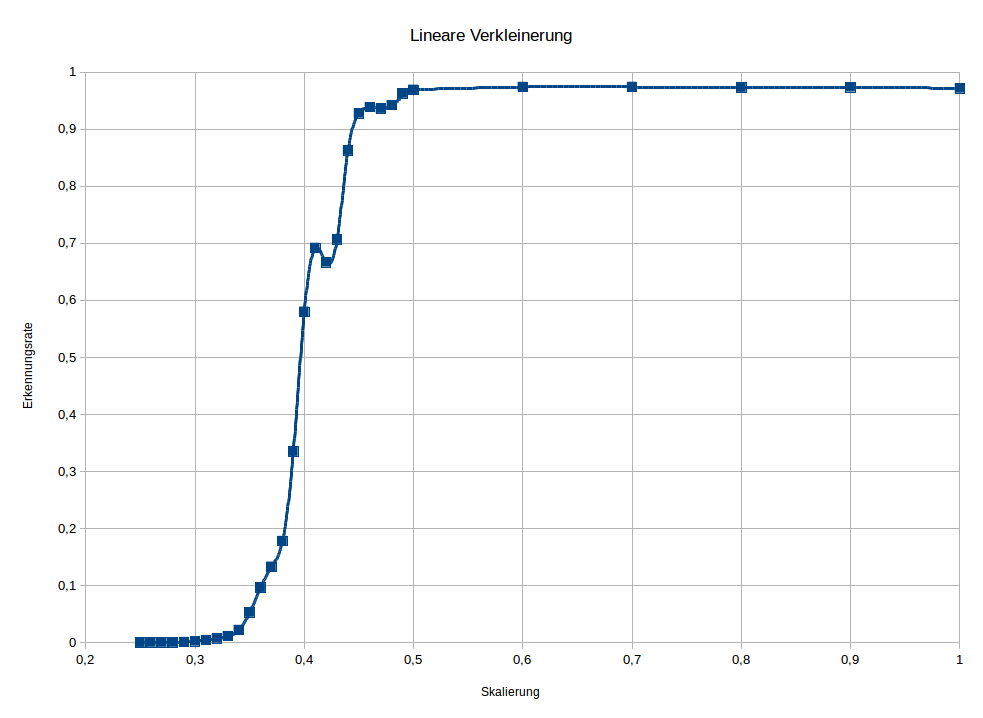
\includegraphics[width=0.45\linewidth]{img/lineare_Verkleinerung}
	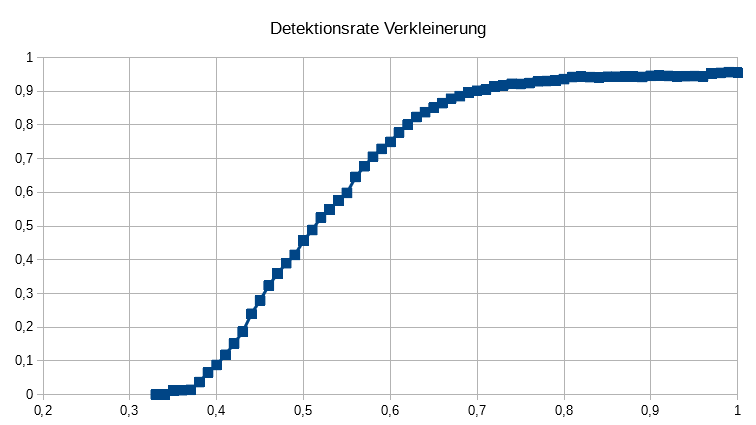
\includegraphics[width=0.45\linewidth]{img/lineare_Verkleinerung2}
	\caption{Die Bilder aus Labeled Faces in the Wild \cite{database_Face} (links) und Random Forests \cite{database_Face_Ori} wurden mit den Faktor auf der X-Achse linear verkleinert und die Erkennungsrate Y-Achse abgebildet}
	\label{img_lineareverkleinerung}
\end{figure}
Es ist zu erkennen, dass die Wahrscheinlichkeit auf eine erfolgreiche Detektion ab $0.5$, also etwa Gesichert mit 47 Pixel Breite, rapide abnimmt. Bei der verwendeten Kamera \autoref{hardware} entspricht dies einer Distanz von etwa $4.5m$.\\
Bei der maximalen Distanz auf der gearbeitet werden soll $(8.5m)$ ergibt sich eine Gesichtsgröße von etwa 22 Pixel, das einer Skalierung von 0.25 entspricht. Bei dieser Bildgröße ist keine Detektion möglich, siehe \autoref{img_lineareverkleinerung}.
\subsection{verschiedenen Skalierungesverfahren}
Um auf den gewünschten Distanzen arbeiten zu können, wird der jeweilige Bereich Hochskaliert. Dazu wird das Ursprüngliche Bild $(250\times 250)$ linear um den angegebene Faktor verkleinert und anschließend mit den angegebenen Verfahren auf $300\times 300$ wieder vergrößert. Die Wahrscheinlichkeit auf eine Detektion ist in \autoref{img_hochskalliern} abgebildet.\\
\begin{figure}
	\centering
	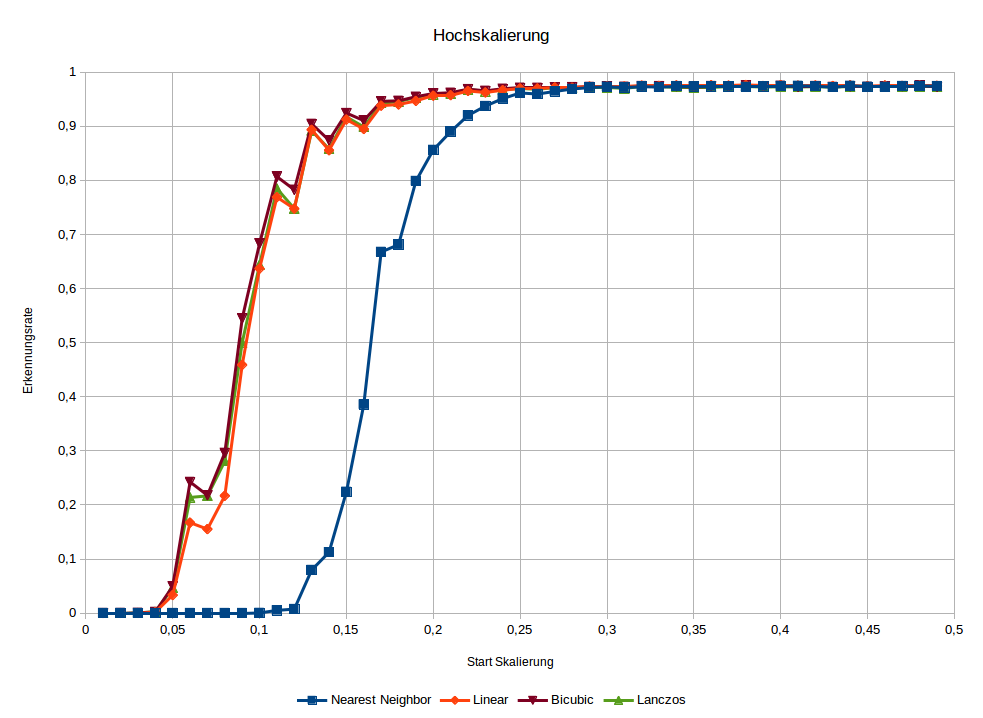
\includegraphics[width=0.5\linewidth]{img/Hochskalliern}
	\caption{Die Bilder aus Labeled Faces in the Wild \cite{database_Face} wurden mit den Faktor auf der X-Achse linear verkleinert und mit den verschiedenen Verfahren wieder vergrößert \autoref{scale_Algos}. Aufgetragen gegen die Detektionswahrscheinlichkeit.
	Nearest-Neighbor (blau), Linear (rot), Bicubic (braun), Lanczos (grün)}
	\label{img_hochskalliern}
\end{figure}
Es ist zu erkennen das durch die Vergrößerung, Gesichter in Bereichen die normal nicht erkennbar sind, bestimmbar werden. Als das ungeeignetste Verfahren hat sich Nearest-Neighbor herausgestellt, siehe blaue Linie \autoref{img_hochskalliern}. Die anderen haben sehr ähnliche Ergebnisse, nur das Lineare Verfahren ist etwas schlechter. Dennoch werden die Anforderungen, einer Detektion auf Gesichtern von 22 Pixel (Skalierung 0.25) von allen erfüllt.\\
Ausgehend vom Skalierungsfaktor des Linearen-, Bicubic- und Lanczos-Verfahren wären mit der verwendeten Kamera auch Distanzen bis zu $14m$ möglich. Allerdings ist das Bild durch die Verkeilung  deutlich besser als Originalaufnahmen, da Pixelrauschen nicht vorhanden ist.
\subsection{Pixelrauschen bei den Skalierungesverfahren}
Um Pixelrauchen zu simulieren, wurden die Bilder aus Labeled Faces in the Wild \cite{database_Face} entsprechend verkleinert und dann mit Rauschen versehen um sie anschließend mit den verschiedenen Verfahren zu vergrößern.\\
Somit soll geprüft werden, welches der Verfahren auch stabil gegen Rauschen ist.
\begin{figure}
	\centering
	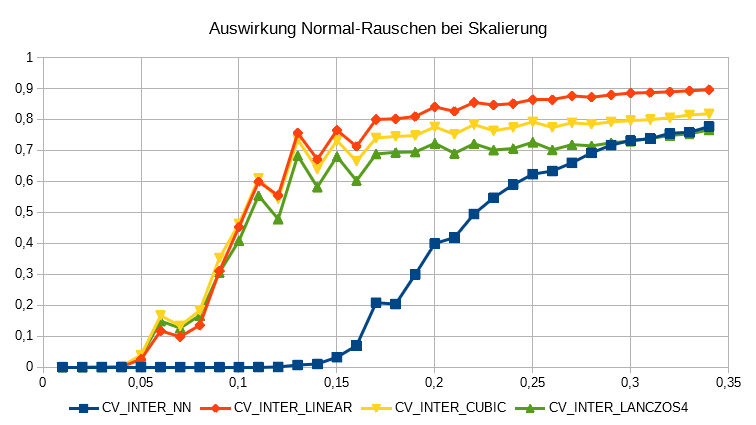
\includegraphics[width=0.7\linewidth]{img/Hochskalliern_Nois}
	\caption{Bilder aus Labeled Faces in the Wild \cite{database_Face}, mit dem X-Faktor verkleinert, um jedes Pixel mit $50\%$ Wahrscheinlichkeit auf $\pm 10\%$ Gleichverteilung der Abweichung}
	\label{img_hochskalliern_nois}
\end{figure}
Das Rauschen wird für jedes Pixel mit einer Wahrscheinlichkeit von $50\%$ auf eine gleich verteilte Abweichung von $\pm 10\%$ des Originalen Farbwertes simuliert. Anschließend wird das verrausche Bild mit den verschiedenen Verfahren vergrößert. Dieser Vorgag wurde für jedes Bild vier mal wiederholt um Zufälligkeiten zu vermeiden.\\
Wie zu erwarten ist Nearest-Neighbor am schlechtesten, aber auch zwischen den anderen Verfahren sind nun unterscheiden zu erkennen, die gesamte Erkrankungsrate ist signifikant kleiner als ohne Rauschen, wobei die Position $(0.15)$ ab der die Erkennungsrate rapide abfällt beibehalten wird.
\subsection{Auswirkung von Pixelrauschen}
Durch Aufnahme eines Schwarzbildes der Actioncam zeigt sich, dass das Pixelrauschen recht hoch ist, siehe \autoref{img_noishight}. Das Rauschen hat keine Normalverteilung, sondern es besteht aus kleinen Bereiche, die den selben fehlerhaften Farbwert besitzen.
\begin{figure}
	\centering
	\fbox{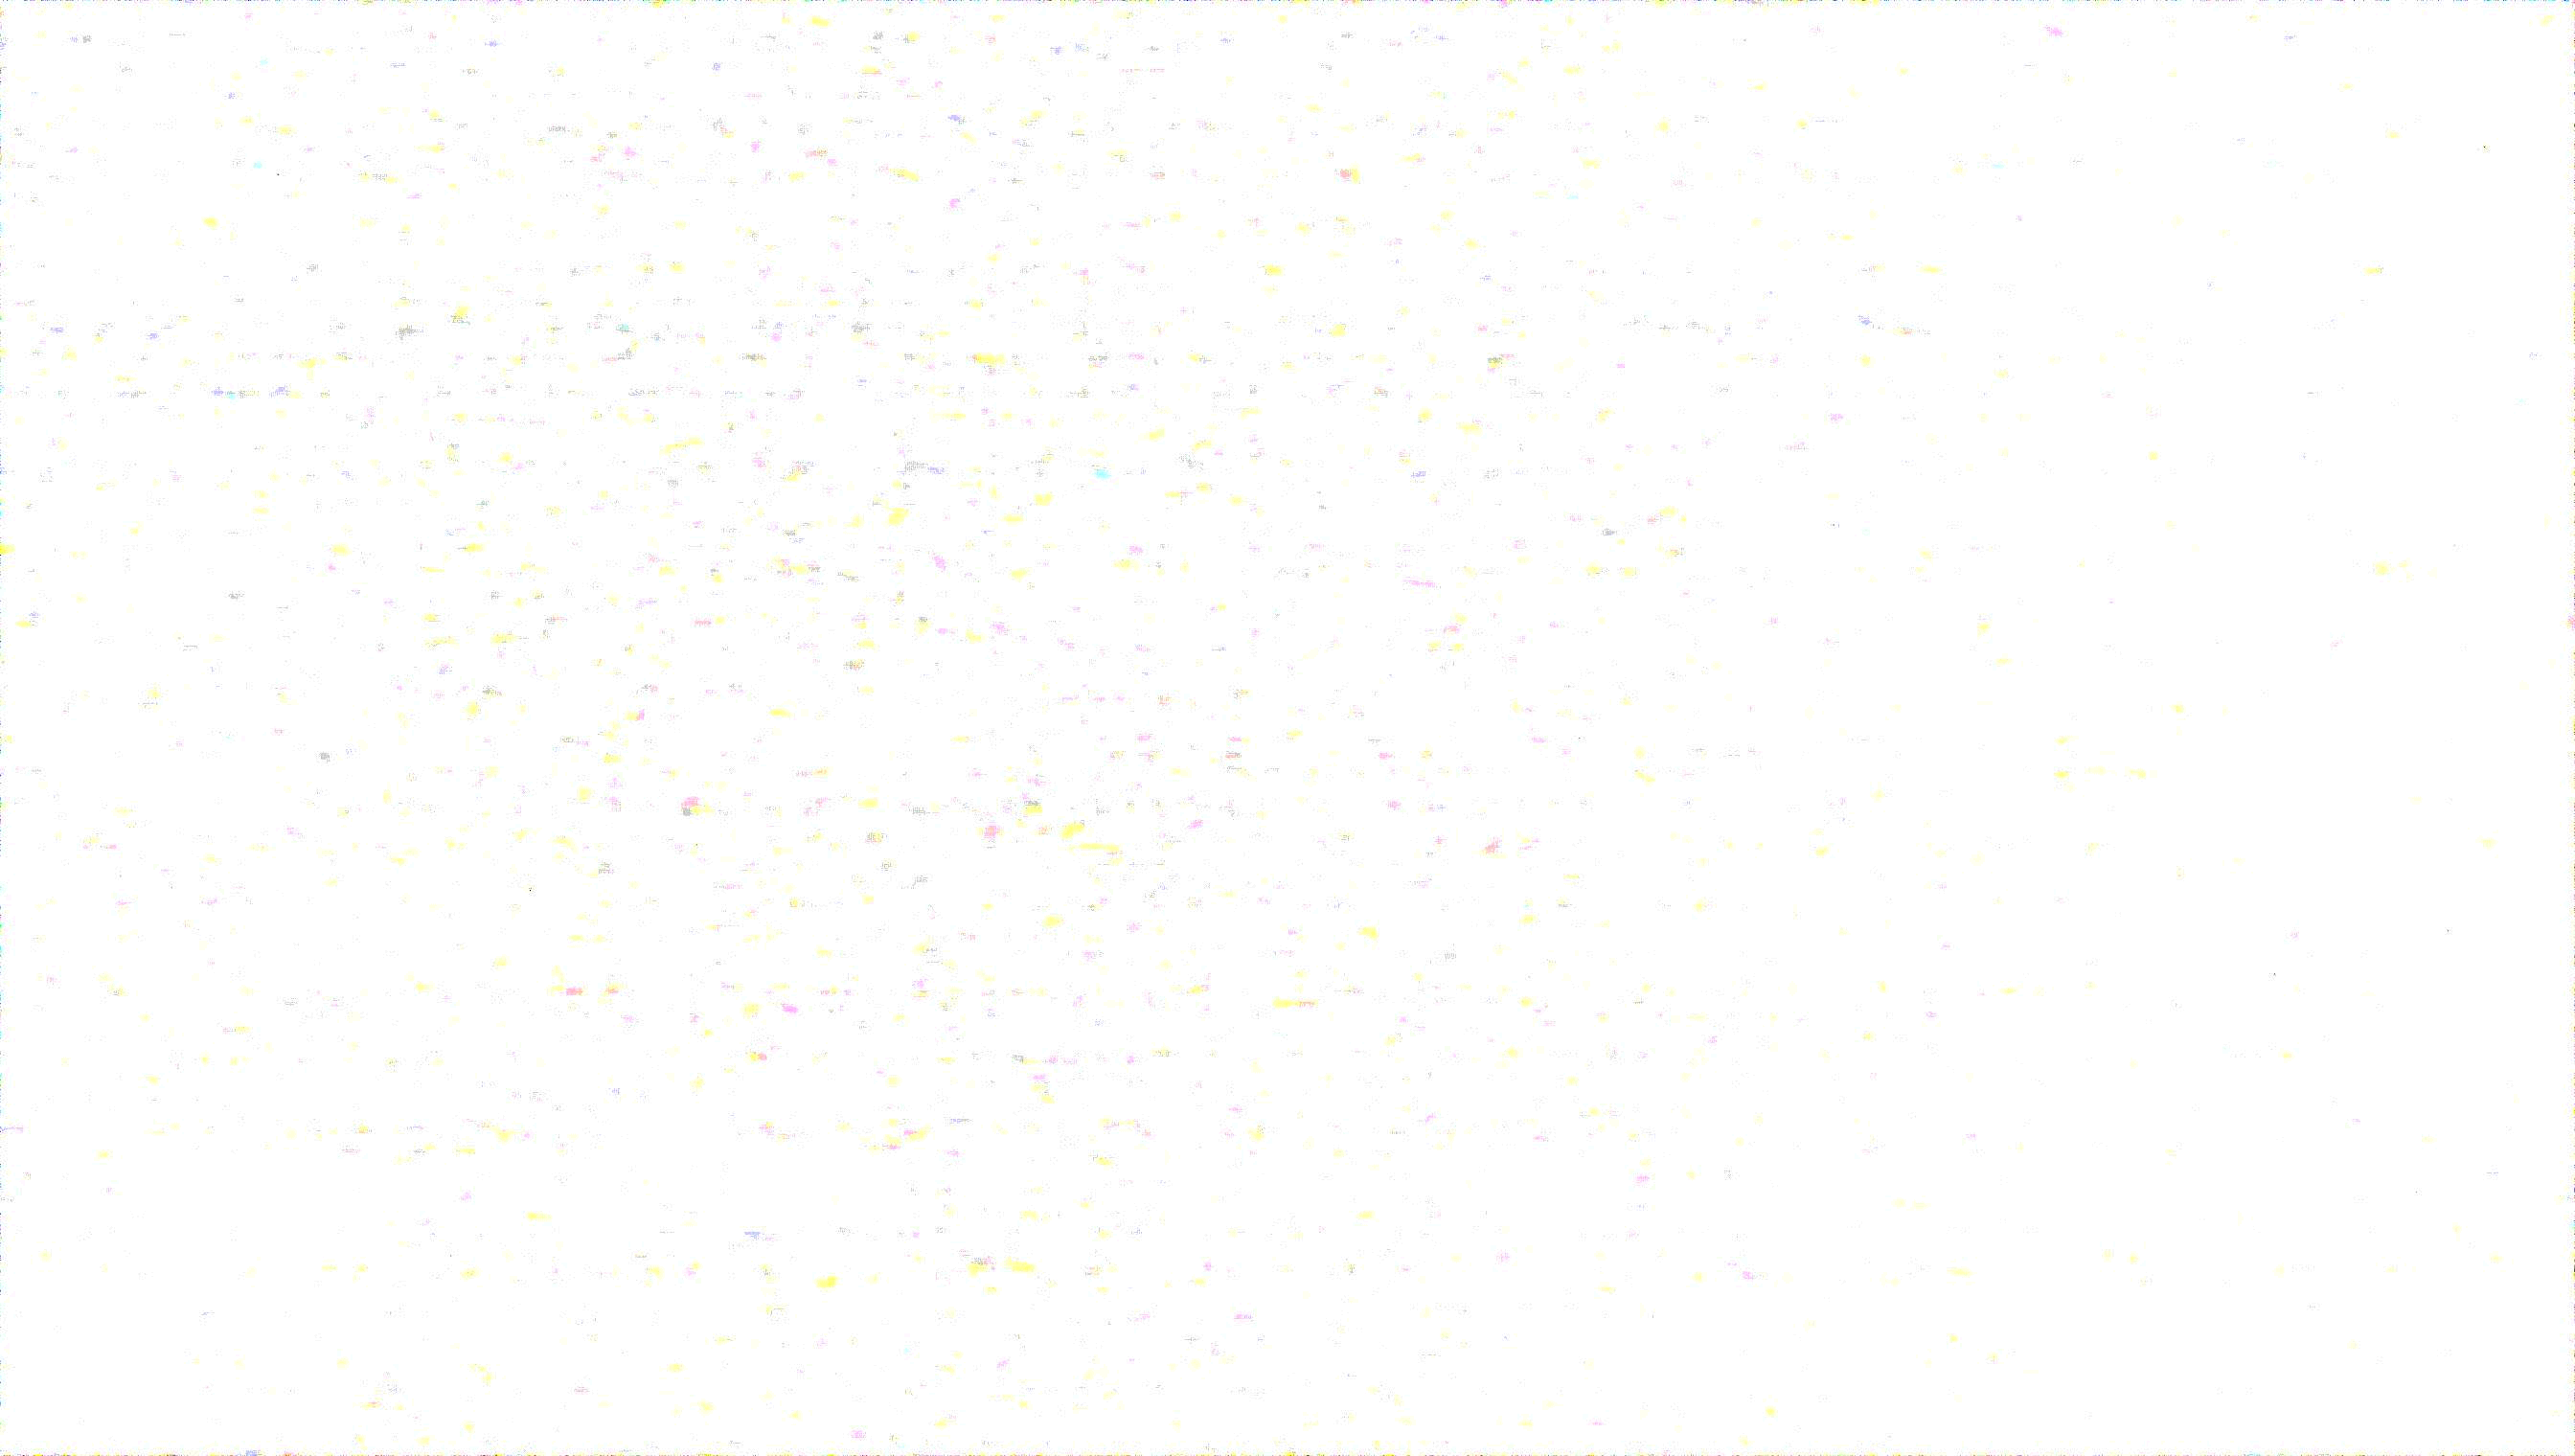
\includegraphics[width=1\linewidth]{img/NoisHight}}
	\caption{Aufnahme eines Schwarz-Bildes $(2688\times 1520)$ der Actioncam um den Faktor 7 verstärkt und invertiert.}
	\label{img_noishight}
\end{figure}
\subsection{Größe und Genauigkeit}
Um die Qualität auf verschiedenen Distanzen zu ermitteln, wurde der Datensatz Forests for Real Time 3D Face Analysis \cite{database_Face_Ori} verwendet, da für jedes Gesicht sein Position und Orientierung bekannt ist. Um die verschiedenen Ditanzen würden die Bilder mit dem angegebene Faktor (X-Achse) verkleinert und mit dem Original verglichen.\\
Da verschiedene Verfahren angeboten werden zur Bestimmung der Position und Orientierung, werden diese miteinander verglichen, siehe \autoref{img_X_Pos}. Zur Bestimmung wurde nur das RGB-Bild verwendet und nich zusätzlich die Tiefeinaufnahme, da dies in der Anwendung auch nicht vorhanden sind.\\
Es zeigt sich, dass Pose World, also die einfache Bestimmung der Position mittels Skalierungsfaktor und zusätzlicher Korrektur der Wikel die besten Ergebnisse liefert.\\
Die Bestimmung mittels der Überführung von 3D zu 2D Punkten ist nicht notwendig,da ein schlechteres Ergebnis erzieht wurde.
\subsubsection{Position}
Zur Bestimmung der Position gibt es zwei Verfahren, die direkte mittels Brennweite und Skalierung oder die Überführungsmatrix von den 3D und 2D Landmarks.\\
\begin{figure}
	\centering
	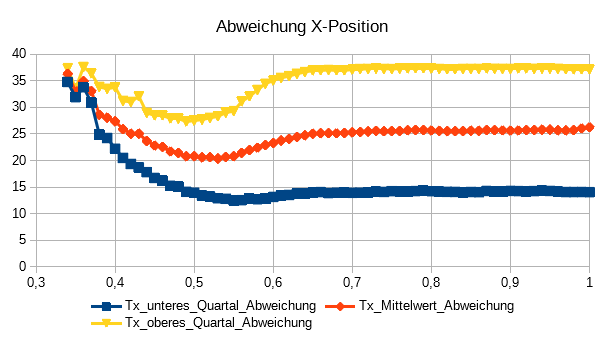
\includegraphics[width=0.45\linewidth]{tabelle/X_Pos_PC}
	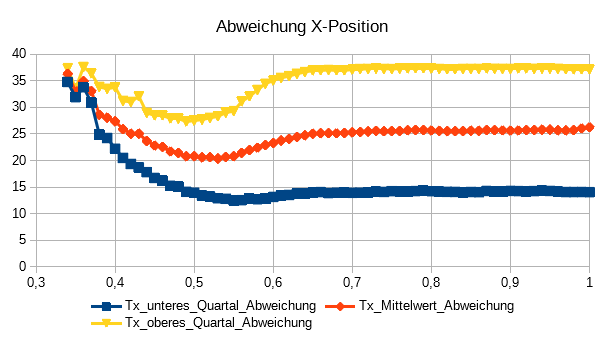
\includegraphics[width=0.45\linewidth]{tabelle/X_Pos_PW}
	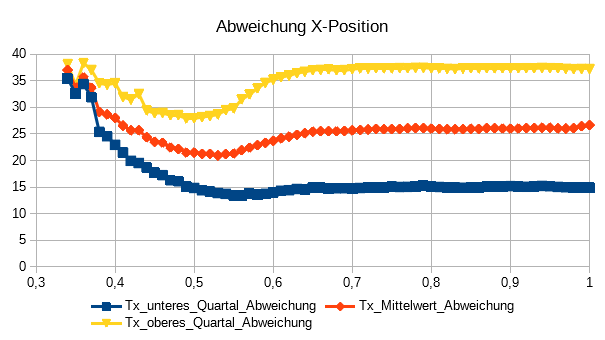
\includegraphics[width=0.45\linewidth]{tabelle/X_Pos_CPC}
	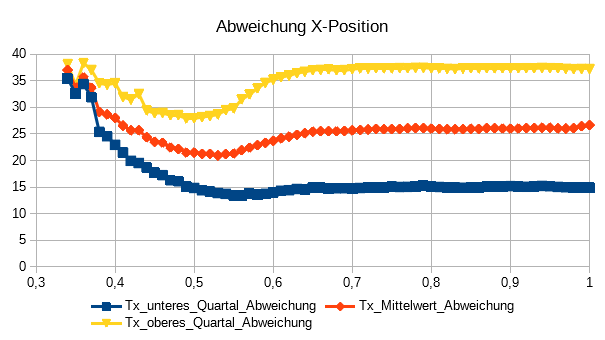
\includegraphics[width=0.45\linewidth]{tabelle/X_Pos_CPW}
	\caption{Pose World (links oben), Pose World (rechts oben), Correct Pose Camera (links unten) und Coorect Pose World, der Abstand (Y-Achse) ist in Millimeter.}
	\label{img_X_Pos}
\end{figure}
Die Funktionen Pose Camera und Pose World (Obere in \autoref{img_X_Pos}) verwenden die einfache Bestimmung mittels Skalierung. Dargestellt ist nur die X-Werte, da die Y-Werte eine recht ähnliche Verteilung liefern.\\
Bei den Z-Werten ergibt sich ein etwas anderer Verlauf, bei dem allerdings sie Fehlerquote bei kleinen Bildern gut sichtbar wird, siehe \autoref{img_Z_Pos}.\\
\begin{figure}
	\centering
	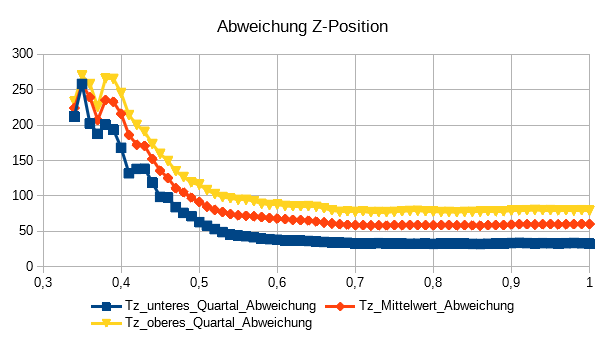
\includegraphics[width=0.45\linewidth]{tabelle/Z_Pos_PC}
	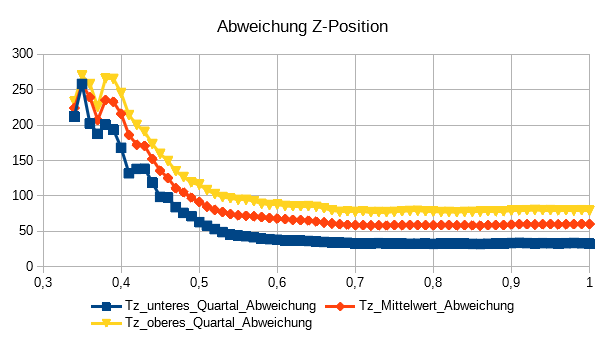
\includegraphics[width=0.45\linewidth]{tabelle/Z_Pos_PW}
	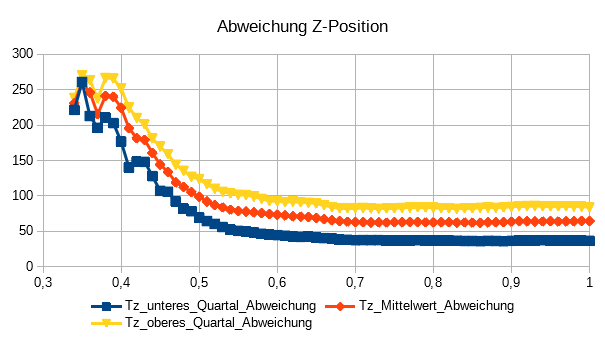
\includegraphics[width=0.45\linewidth]{tabelle/Z_Pos_CPC}
	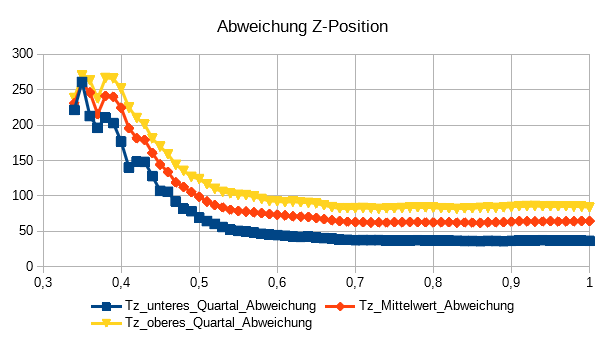
\includegraphics[width=0.45\linewidth]{tabelle/Z_Pos_CPW}
	\caption{Pose World (links oben), Pose World (rechts oben), Correct Pose Camera (links unten) und Coorect Pose World, der Abstand (Y-Achse) ist in Millimeter.}
	\label{img_Z_Pos}
\end{figure}
Zur Bewertung, die Durchschnittliche Distanz zwischen Kamera und Kopf beträgt ca $70cm$ bei einer Kopfbreite von 78 Pixel. Der schnelle Abfall der Genauigkeit ist an der selben stelle (0.5) an der auch die Detektionsrate stark absinkt.
\subsubsection{Orientierung}
Auch bei der Orientierung werden die verscheiden Methoden miteinander verglichen. Die Analyse hat gezeigt, dass die Qualität der Verfahren von den einzelnen Rotationen abhängt.\\
\begin{figure}
	\centering
	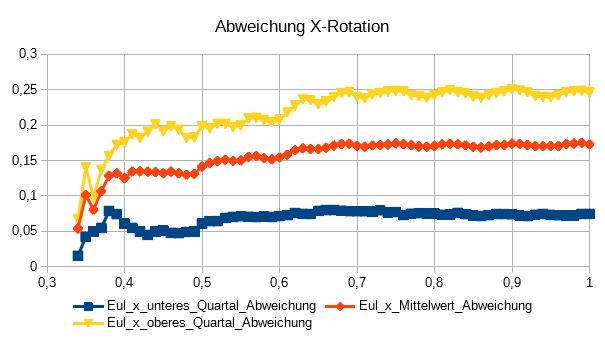
\includegraphics[width=0.45\linewidth]{tabelle/X_Rot_PC}
	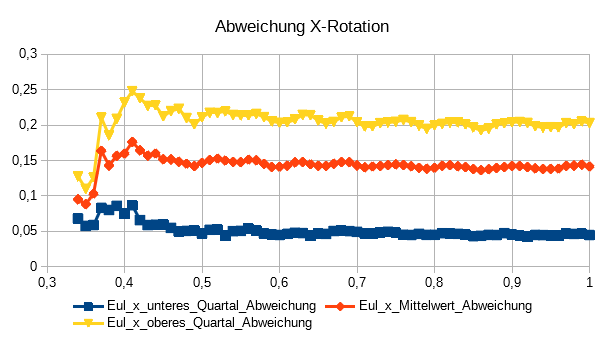
\includegraphics[width=0.45\linewidth]{tabelle/X_Rot_PW}
	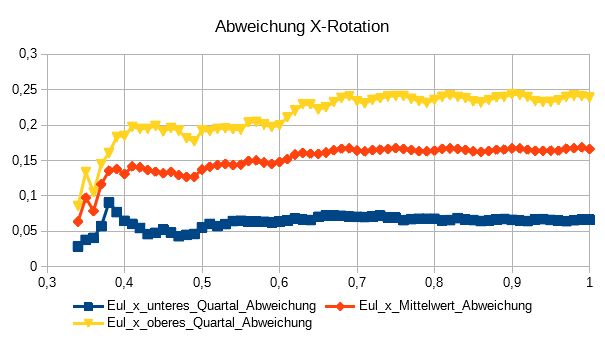
\includegraphics[width=0.45\linewidth]{tabelle/X_Rot_CPC}
	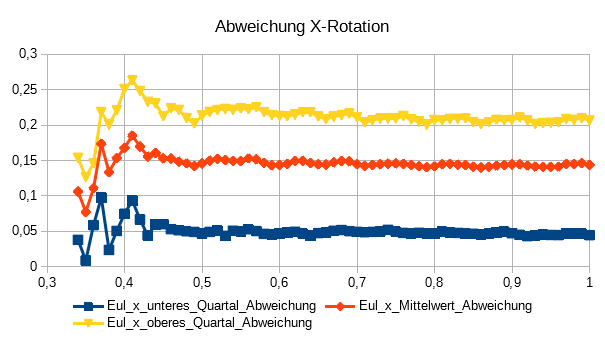
\includegraphics[width=0.45\linewidth]{tabelle/X_Rot_CPW}
	\caption{Pose World (links oben), Pose World (rechts oben), Correct Pose Camera (links unten) und Coorect Pose World, der Abstand (Y-Achse) ist im Bogenmaß.}
	\label{img_X_Pot}
\end{figure}
Bei der X-Rotation, dargestellt in \autoref{img_X_Pot} können die rechten Verfahrenen (Pos World und Correct Pose World) überzeugen. Vor alle, Pose World hat selbst bei kleinen Abbildungen nur eine mittlere Abweichung von $8.5^\circ$\\
\begin{figure}
	\centering
	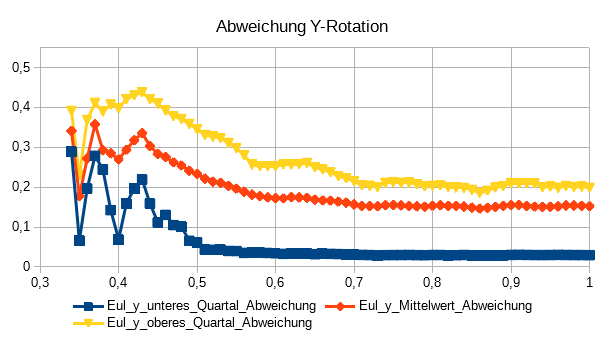
\includegraphics[width=0.45\linewidth]{tabelle/Y_Rot_PC}
	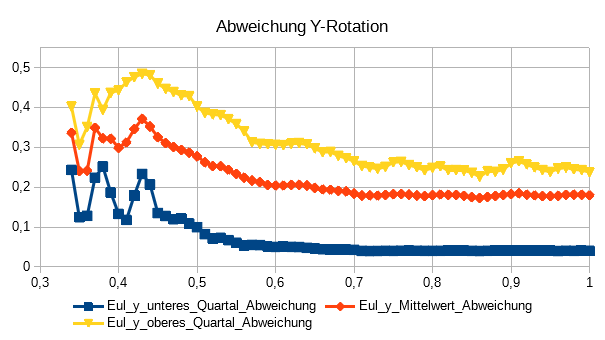
\includegraphics[width=0.45\linewidth]{tabelle/Y_Rot_PW}
	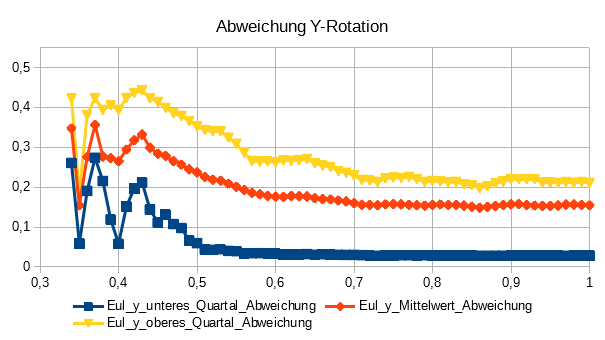
\includegraphics[width=0.45\linewidth]{tabelle/Y_Rot_CPC}
	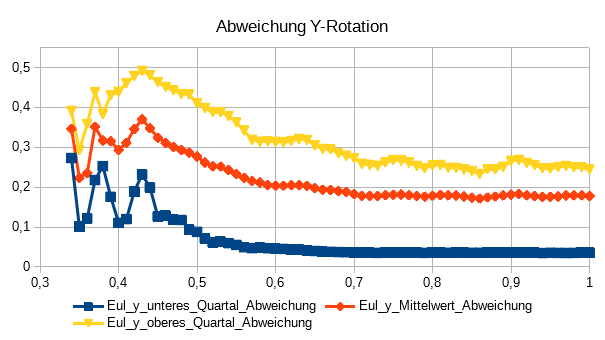
\includegraphics[width=0.45\linewidth]{tabelle/Y_Rot_CPW}
	\caption{Pose World (links oben), Pose World (rechts oben), Correct Pose Camera (links unten) und Coorect Pose World, der Abstand (Y-Achse) ist m Bogenmaß.}
	\label{img_Y_Pot}
\end{figure}
Um die Y-Rotation zu ermitteln ist nun allerdings die linken (Pose Came und Correct Pose Came) den rechten (Posw Worls und Correcht Pose World) deutlich überlegen, siehe \autoref{img_Y_Pot}. Auch hier liegt der mittlere Fehler über lange Zeit bei etwa $9^\circ$\\
\begin{figure}
	\centering
	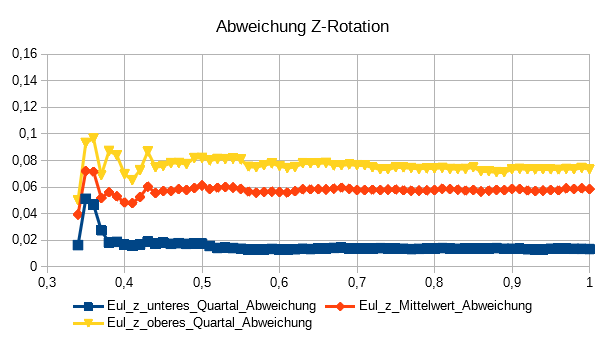
\includegraphics[width=0.45\linewidth]{tabelle/Z_Rot_PC}
	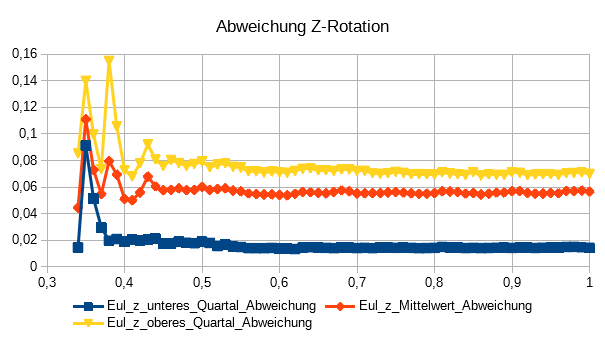
\includegraphics[width=0.45\linewidth]{tabelle/Z_Rot_PW}
	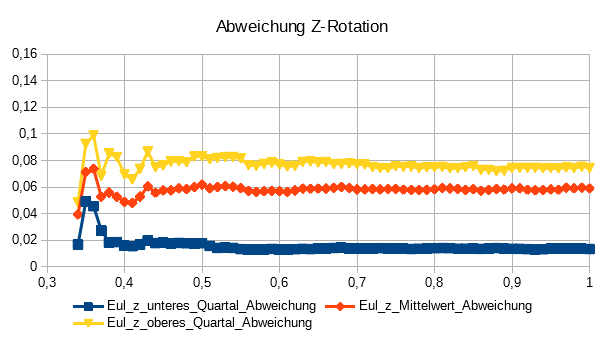
\includegraphics[width=0.45\linewidth]{tabelle/Z_Rot_CPC}
	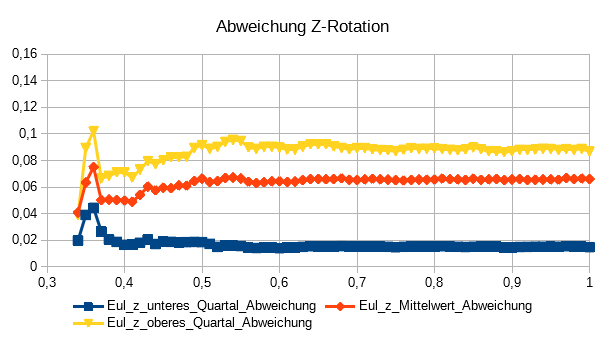
\includegraphics[width=0.45\linewidth]{tabelle/Z_Rot_CPW}
	\caption{Pose World (links oben), Pose World (rechts oben), Correct Pose Camera (links unten) und Coorect Pose World, der Abstand (Y-Achse) ist im Bogenmaß.}
	\label{img_Z_Pot}
\end{figure}
Bei der Bestimmung von der Z-Rotation sind die Correct Pose Came und Pose Came nahe zu gleich gut, Correkt Pose World allerding schlechter und Pose World besser, siehe \autoref{img_Z_Pot}. Wobei auffällt, dass Pose World bei Werten unter 0.4 plötzlich sehr schlecht wird.
\subsubsection{Wertebereich Rotation}
Von Interesse sind auch die Winkel, bei den Gesichter in verschiedenen Skalierungen noch erkannt werden, siehe \autoref{img_Rot_Value}.\\
Hier ist zu erkennend das der Wertebereich ab 0.7 abnimmt und ab 0.5 recht schnell. Dies ist wichtig zu wissen, da wenn kein gesicht in diesen Bereichen nicht erkannt werden kann auch die späteren Verfahren nicht bestimmt werden können.\\
Der Wertebereich auf den einzelnen Achsen sollte ist ausreichend sein für die Anwendung, auch wenn die Rotation pralle zur Horizontalen etwas größer sein könnte.
\begin{figure}
	\centering
	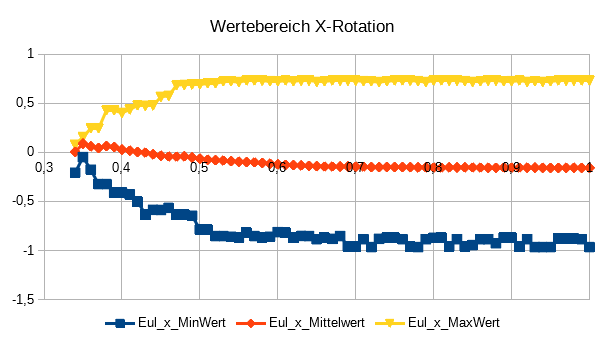
\includegraphics[width=0.3\linewidth]{tabelle/X_Rot}
	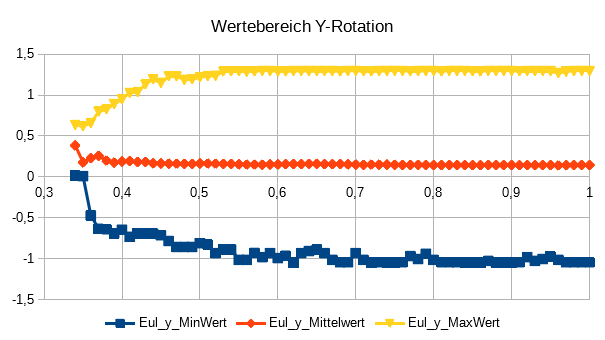
\includegraphics[width=0.3\linewidth]{tabelle/Y_Rot}
	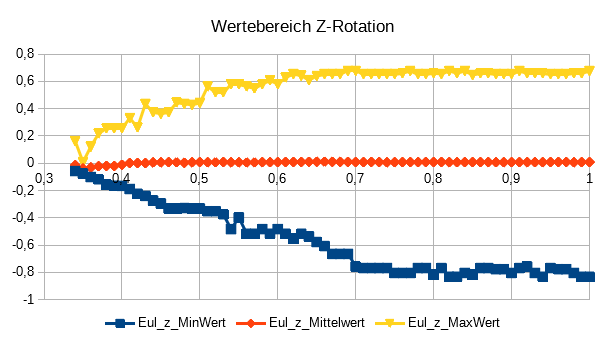
\includegraphics[width=0.3\linewidth]{tabelle/Z_Rot}
	\caption{Darstellung der noch detektierten Wertebereiche in Bogenmaß.}
	\label{img_Rot_Value}
\end{figure}
\subsection{Qualität der Skalierung}
Nun wird der Zusammenhang zwischen den verscheiden Skalierungsverfahren und der Qualität der Ergebnisse gesucht.\\
Es zeigt sich, dass bei der Bestimmung der Parameter ist das Nearest-Neighbor Verfahren am genauesten, allerdings sit der Wertebereich deutlich eingeschränkt, die Mindestgröße des Gesichts im Orginal und den geringer Wertebereich bei den Rotationen ist dieses Verfahren eher ungeeignet.\\
Bei dem Linearen Verfahren ist die Abweichung bei den Rotationen am größten, auch wenn es sich nur um etwa ein halbes Grad handelt. Zwischen dem Bicubic- und Lanczos-Verfahren gibt es in den relevanten Bereichen keinen signifikanten Unterschied, wobei das Lanczos in den kleineren Bereichen gleichmäßigere Ergebnisse, kann aber vom Rechenaufwand abhängig gemacht werden welches Verfahren gewählt werden soll. 
\subsubsection{Position}
Als erstes wird die berechnete Distanz miteinander verglichen.
\begin{figure}
	\centering
	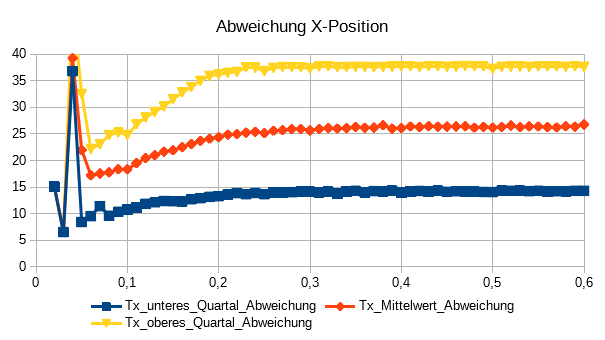
\includegraphics[width=0.45\linewidth]{tabelle2/X_Pos_Cubic}
	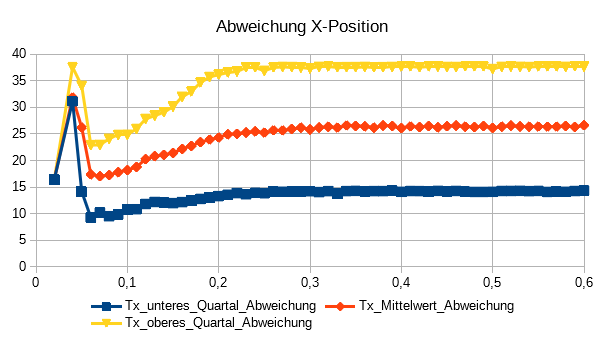
\includegraphics[width=0.45\linewidth]{tabelle2/X_Pos_Lanc}
	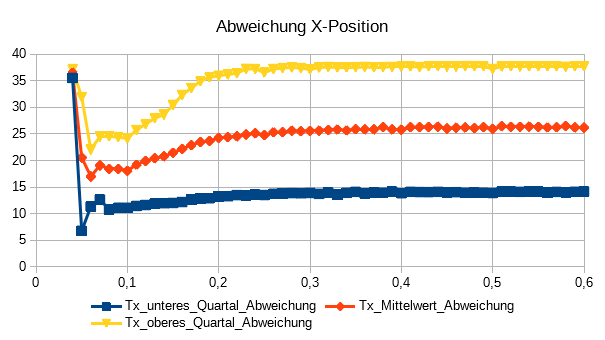
\includegraphics[width=0.45\linewidth]{tabelle2/X_Pos_Linear}
	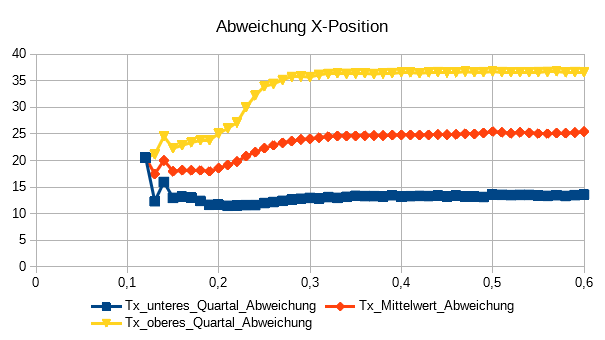
\includegraphics[width=0.45\linewidth]{tabelle2/X_Pos_NN}
	\caption{Zusammenhang zwischen der Skalierung (X-Achse) und der Abweichung in X-Richtung (Y-Achse) in Millimeter. 
	 Bicubic (oben links), Lanczos (oben rechts), Linear (unten links), Nearest-Neighbor (unten rechts)}
	\label{img_X_Pos_Skal}
\end{figure}
 In \autoref{img_X_Pos_Skal} ist die Abweichung entlang der X-Achse dargestellt. Nearest-Neighbor liefert die besten Ergebnise, auch wenn durch die schlechtere Detektionsrate dieses Verfahren früher ausfällt als die anderen drei.\\
\begin{figure}
	\centering
	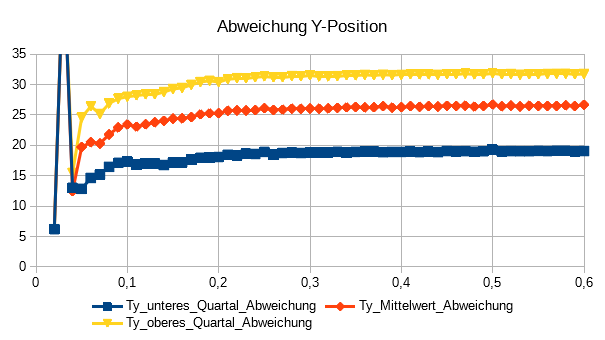
\includegraphics[width=0.45\linewidth]{tabelle2/Y_Pos_Cubic}
	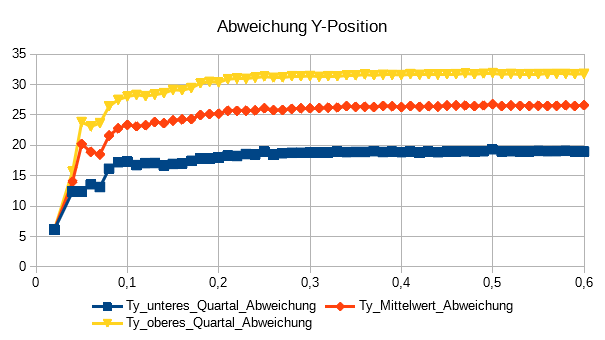
\includegraphics[width=0.45\linewidth]{tabelle2/Y_Pos_Lanc}
	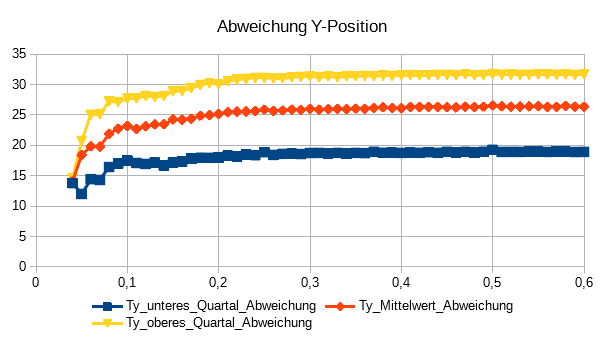
\includegraphics[width=0.45\linewidth]{tabelle2/Y_Pos_Linear}
	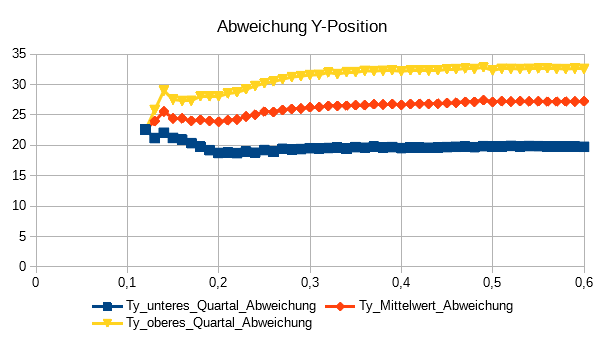
\includegraphics[width=0.45\linewidth]{tabelle2/Y_Pos_NN}
	\caption{Zusammenhang zwischen der Skalierung (X-Achse) und der Abweichung in Y-Richtung (Y-Achse) in Millimeter. 
		Bicubic (oben links), Lanczos (oben rechts), Linear (unten links), Nearest-Neighbor (unten rechts)}
	\label{img_Y_Pos_Skal}
\end{figure}
Auf der Y-Achse ist das Lineare-Verfahren etwas besser als die Andren, das Nearest-Neighbor ist hierbei überraschend das Schlechteste, siehe \autoref{img_Y_Pos_Skal}.\\
\begin{figure}
	\centering
	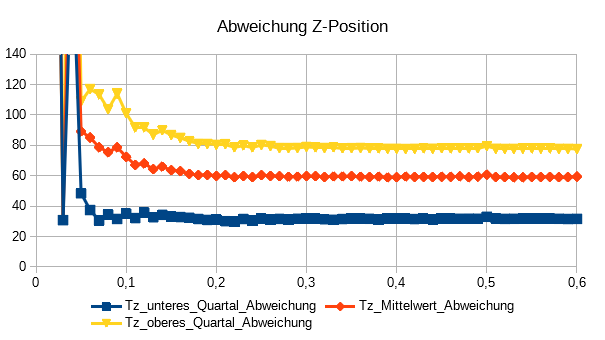
\includegraphics[width=0.45\linewidth]{tabelle2/Z_Pos_Cubic}
	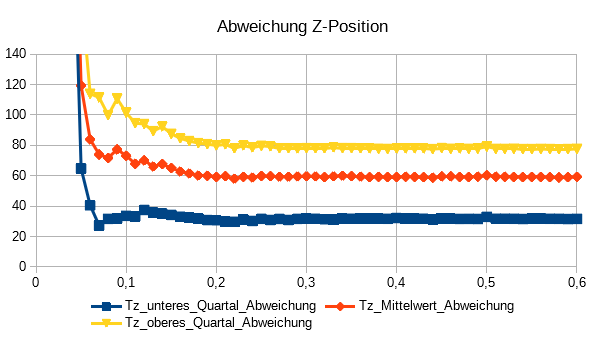
\includegraphics[width=0.45\linewidth]{tabelle2/Z_Pos_Lanc}
	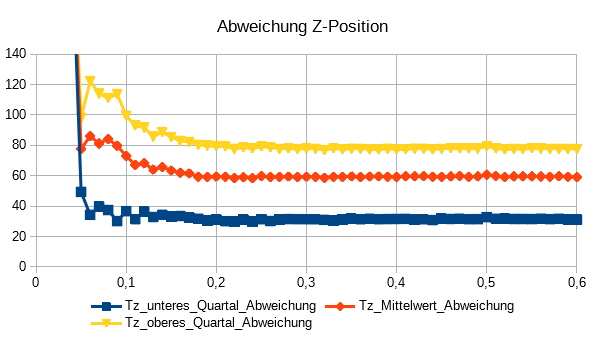
\includegraphics[width=0.45\linewidth]{tabelle2/Z_Pos_Linear}
	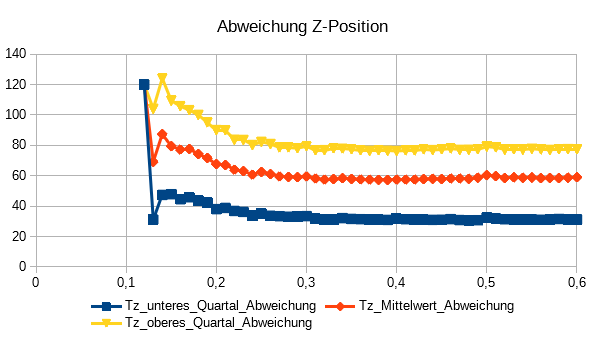
\includegraphics[width=0.45\linewidth]{tabelle2/Z_Pos_NN}
	\caption{Zusammenhang zwischen der Skalierung (X-Achse) und der Abweichung in Z-Richtung (Y-Achse) in Millimeter. 
		Bicubic (oben links), Lanczos (oben rechts), Linear (unten links), Nearest-Neighbor (unten rechts)}
	\label{img_Z_Pos_Skal}
\end{figure}
Nur schwer zu erkennen, da der Unterschied nur minimal ist, ist auch hier das  Nearest-Neighbor  genauer, siehe \autoref{img_Y_Pos_Skal}. Die anderen drei sind nahezu identisch. Bei sehr kleinen Skalierungen existieren durchaus auch sehr große Fehler, diese wurden allerdings bei der Darstellung abgeschnitten, da bei dieser Größe die Detektionsrate so klein ist, dass sie nahezu irrelevant werden.
\subsubsection{Orientierung}
Als weitere Bestimmung wird die berechneten Winkel um die jeweilige Achse.
\begin{figure}
	\centering
	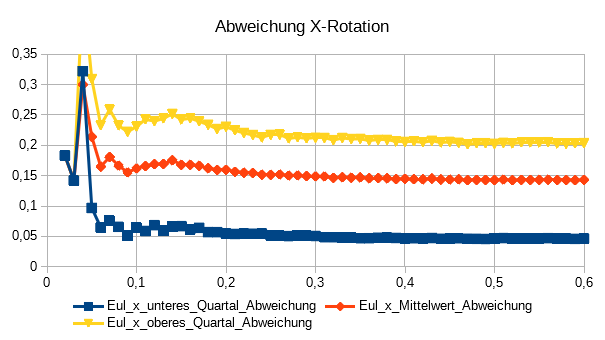
\includegraphics[width=0.45\linewidth]{tabelle2/X_Rot_Cubic}
	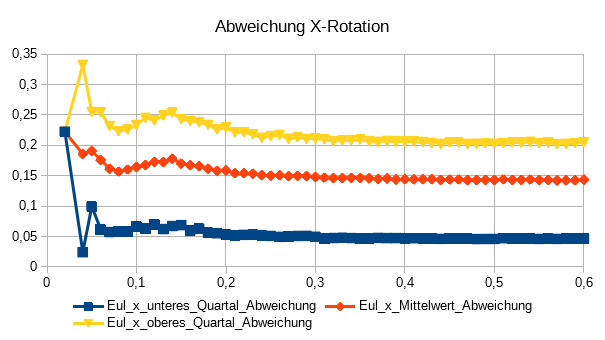
\includegraphics[width=0.45\linewidth]{tabelle2/X_Rot_Lanc}
	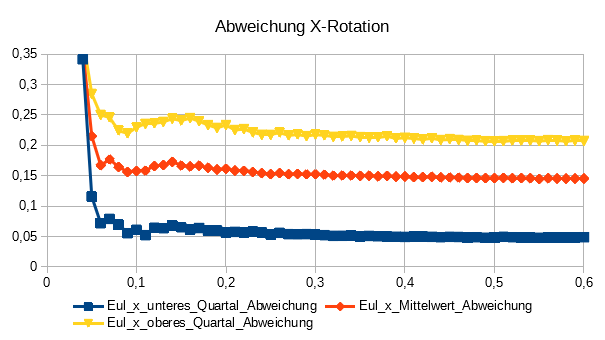
\includegraphics[width=0.45\linewidth]{tabelle2/X_Rot_Linear}
	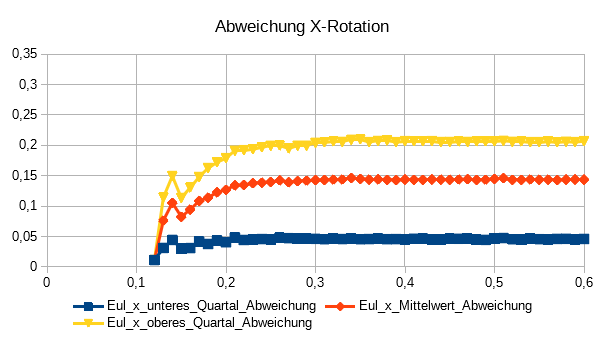
\includegraphics[width=0.45\linewidth]{tabelle2/X_Rot_NN}
	\caption{Zusammenhang zwischen der Skalierung (X-Achse) und der Abweichung des Winkels in X-Richtung, Angabe in Bogenmaß. 
		Bicubic (oben links), Lanczos (oben rechts), Linear (unten links), Nearest-Neighbor (unten rechts)}
	\label{img_X_Rot_Skal}
\end{figure}
\begin{figure}
	\centering
	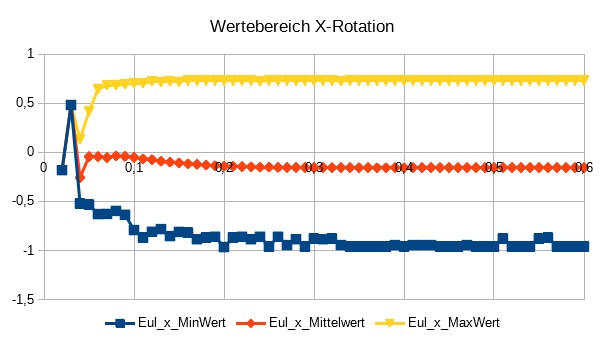
\includegraphics[width=0.45\linewidth]{tabelle2/X_Rot_Val_Cubic}
	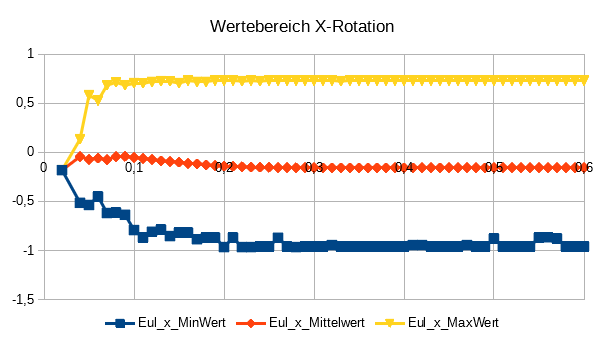
\includegraphics[width=0.45\linewidth]{tabelle2/X_Rot_Val_Lanc}
	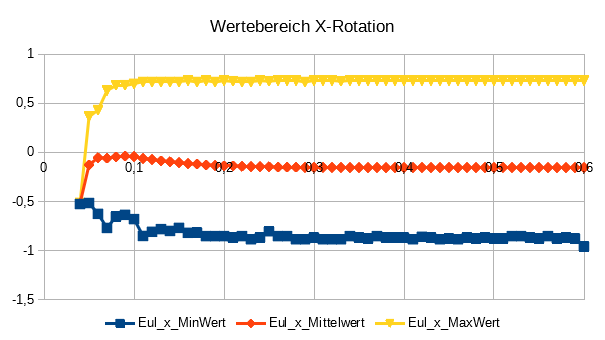
\includegraphics[width=0.45\linewidth]{tabelle2/X_Rot_Val_Linear}
	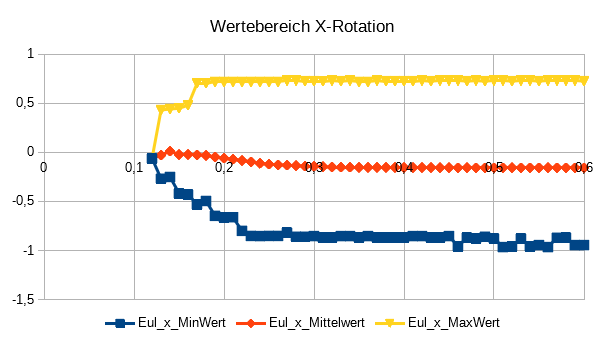
\includegraphics[width=0.45\linewidth]{tabelle2/X_Rot_Val_NN}
	\caption{Zusammenhang zwischen der Skalierung (X-Achse) und der Abweichung des Winkels in X-Richtung, Angabe in Bogenmaß. 
		Bicubic (oben links), Lanczos (oben rechts), Linear (unten links), Nearest-Neighbor (unten rechts)}
	\label{img_X_Rot_Val_Skal}
\end{figure}
Geringste Abweichung bei der bestimung der X-Rotation bei Nearest-Neighbor, siehe \autoref{img_X_Rot_Skal}. Auffällig ist außerdem der kleinere Wertebereich des Linearen-Verfahrens.\\
\begin{figure}
	\centering
	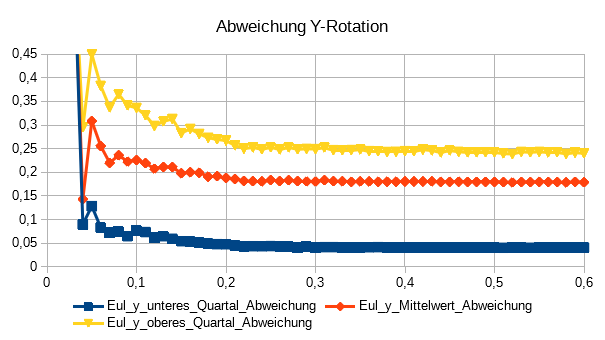
\includegraphics[width=0.45\linewidth]{tabelle2/Y_Rot_Cubic}
	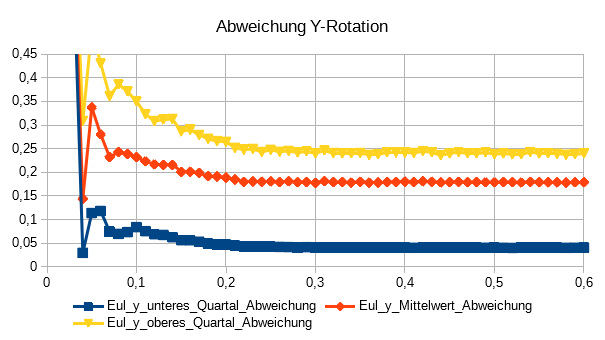
\includegraphics[width=0.45\linewidth]{tabelle2/Y_Rot_Lanc}
	\includegraphics[width=0.45\linewidth]{tabelle2/Y_Rot_Linear}
	\includegraphics[width=0.45\linewidth]{tabelle2/Y_Rot_NN}
	\caption{Zusammenhang zwischen der Skalierung (X-Achse) und der Abweichung des Winkels in Y-Richtung, Angabe in Bogenmaß.
		Bicubic (oben links), Lanczos (oben rechts), Linear (unten links), Nearest-Neighbor (unten rechts)}
	\label{img_Y_Rot_Skal}
\end{figure}
\begin{figure}
	\centering
	\includegraphics[width=0.45\linewidth]{tabelle2/Y_Rot_Val_Cubic}
	\includegraphics[width=0.45\linewidth]{tabelle2/Y_Rot_Val_Lanc}
	\includegraphics[width=0.45\linewidth]{tabelle2/Y_Rot_Val_Linear}
	\includegraphics[width=0.45\linewidth]{tabelle2/Y_Rot_Val_NN}
	\caption{Zusammenhang zwischen der Skalierung (X-Achse) und der Wertebereich des Winkels in Y-Richtung, Angabe in Bogenmaß.
		Bicubic (oben links), Lanczos (oben rechts), Linear (unten links), Nearest-Neighbor (unten rechts)}
	\label{img_Y_Rot_Val_Skal}
\end{figure}
Auch bei der Y-Rotation schneidet Nearest-Neighbor am besten ab, siehe \autoref{img_Y_Rot_Skal}, allerdings sind die unterscheide minimal.\\
\begin{figure}
	\centering
	\includegraphics[width=0.45\linewidth]{tabelle2/Z_Rot_Cubic}
	\includegraphics[width=0.45\linewidth]{tabelle2/Z_Rot_Lanc}
	\includegraphics[width=0.45\linewidth]{tabelle2/Z_Rot_Linear}
	\includegraphics[width=0.45\linewidth]{tabelle2/Z_Rot_NN}
	\caption{Zusammenhang zwischen der Skalierung (X-Achse) und der Abweichung des Winkels in Z-Richtung, Angabe in Bogenmaß.
		Bicubic (oben links), Lanczos (oben rechts), Linear (unten links), Nearest-Neighbor (unten rechts)}
	\label{img_Z_Rot_Skal}
\end{figure}
\begin{figure}
	\centering
	\includegraphics[width=0.45\linewidth]{tabelle2/Z_Rot_Val_Cubic}
	\includegraphics[width=0.45\linewidth]{tabelle2/Z_Rot_Val_Lanc}
	\includegraphics[width=0.45\linewidth]{tabelle2/Z_Rot_Val_Linear}
	\includegraphics[width=0.45\linewidth]{tabelle2/Z_Rot_Val_NN}
	\caption{Zusammenhang zwischen der Skalierung (X-Achse) und der Wertebereiche des Winkels in Z-Richtung, Angabe in Bogenmaß.
		Bicubic (oben links), Lanczos (oben rechts), Linear (unten links), Nearest-Neighbor (unten rechts)}
	\label{img_Z_Rot_Val_Skal}
\end{figure}
Kein erkennbarer Unterschied zwischen den einzelnen Verfahren. Wobei bei Nearest-Neighbor deutlich früher der Wertebereich sinkt.
\subsection{To Do}
\begin{itemize}
	\item Patch Experts und Optimierungsfunktionen CLM
	\item Auswirkung von Pixelrauschen
	\begin{itemize}
		\item Rauschen der Actioncam bestimmen\\
		Done
		\item Simulation des Rauschens\\
		Add Gaußverteilung auf Image 
	\end{itemize}
\item Angabe des Koordiantansystems
\item Auswerten der Messung
\item Wann ELSE
\item Mittlung Ergebnis / Landmarks
\item Zuverlässigkeit mit Farbkorrektur
\end{itemize}